\documentclass[12pt]{book}

\title{Physics 7B Workbook Supplement}
\author{Compiled by Lenny Evans}
\usepackage{paralist,fullpage,amsmath,epsfig,verbatim,multicol,url,circuitikz}

\raggedbottom

\setcounter{chapter}{-1}

\begin{document}

\maketitle

\noindent {\it This is a compilation many of the problems physics 7B GSIs have given in section between 2013-2014. This text is in no way meant to replace the workbook. The problems here highlight topics that are not covered well in the workbook, and topics that are covered well in the workbook are omitted.  I have compiled this material to be free to use now and always. No one should sell this material or make money from it in any way.\\

\noindent Special thanks to all of the GSIs I have worked with (listed below) for providing the problems and for being wonderful GSIs. I would particularly like to thank Neil Goeckner-Wald, Ben Ponedel, Zach Fisher, and Alex Povilus for their contributions and discussions.\\}


\noindent {\bf 2013-2014 Physics 7B GSIs:} Alex Anderson, Sadegh Asefi, Trevor Bowen, Kolen Cheung, Steve Drapcho, Fang Fang, Zach Fisher, Neil Goeckner-Wald, Ian Hayes, Ammar Husain, Zeinab Jahed, Oliver Jeong, Robert Kealhofer, Chiu-yun Lin, Ruhollah Moussani-Banjoji, Adrian Po, Ben Ponedel, Alex Povilus, Dan Rizzo, Alison Saunders, Cory Schillaci, Chukman So, Aaron Szasz, Alex Takeda, Yuguang Tong, Ziqi Yan, and Shudan Zhong.

\tableofcontents

\chapter{Math}

\noindent This section ``reviews'' the various math concepts that students often have trouble with in this course. We say ``review,'' but some of this may be new, and the stuff that is not new, we may be talking about it in a different way than you did in your calculus classes, so do not worry if you do not understand all of it; that is why we are spending time on this. In addition, this chapter will have more explanation than the later chapters because this is not explained in your book and we would like for you to have something to look back on if you get lost at some point.

 There will be a lot of examples from Newton's law of universal gravitation in this chapter. This is because the equations of mass interactions are extremely similar to the equations of charge interactions. If you have mastered one of them, the other should be easy to learn!

 {\it Note: In this text, we will use $\hat{x}, \hat{y},$ and $\hat{z}$ to represent the unit vectors pointing in the $x,y,$ and $z$ directions. You may be used to writing these as $\hat{i},\hat{j},$ and $\hat{k},$ but these are just different names for the same thing.}

 \pagebreak
 
\section{Small Numbers}

{\it By Alison Saunders and Lenny Evans}

\noindent Most often when using Taylor expansions, your argument $x$ will be “very very small.” Mathematically, that will be represented as something like $x \ll 1$. If that is the case, $x^2$ will be really really really small, and $x^3$ will be even smaller yet. So usually, you can eliminate all terms that go like powers of $x^2$ , $x^3$ , etc.. Often this makes problems much more manageable, and often problems cannot be solved unless you take approximations like this. In this class you will never need to use the general form of Taylor series involving the values of the derivative of a function evaluated at a certain point, so we will not write that here. Instead, here are a few useful expansions that come up extremely often:

\begin{equation*}
 \sin(x) \approx x - \frac{x^3}{3!}
\end{equation*}

\begin{equation*}
 \cos(x) \approx 1-\frac{x^2}{2!}+\frac{x^4}{4!}
 \end{equation*}
 
 \begin{equation*}
  e^x \approx 1+x+\frac{x^2}{2!}+\frac{x^3}{3!}+\frac{x^4}{4!}
 \end{equation*}

 \begin{equation*}
  \ln(1+x) \approx x-\frac{x^2}{2}+\frac{x^3}{3}-\frac{x^4}{4}
 \end{equation*}

 \begin{equation*}
  (1+x)^p \approx 1+px+\frac{p(p-1)}{2!}x^2+\frac{p(p-1)(p-2)}{3!}x^3+\frac{p(p-1)(p-2)(p-3)}{4!}x^4
 \end{equation*}
 
 One thing that often confuses people is, how far do you need to go in these expansions? You usually want the first term that is interesting. For example, think about $\sin(x).$ When $x$ is close to zero, $\sin(x)$ is roughly zero, but that isn't very interesting, as it does not tell us how the answer changes if we change $x.$ So, the more interesting thing to say is $\sin(x)$ looks like $x$ when $x$ is close to zero. The math lingo we use is to say that $\sin(x)$ is {\it asymptotic} to $x$ as $x\to 0.$
 
 We can also think about asymptotic forms when a number gets large. For example, what does a gravitational force between two objects look like as the distance between the two objects is made large? In this case, if the variable growing large is called $x,$ you want to find a Taylor series to take in $1/x.$ If $x$ is large, $1/x$ will be small, so this seems reasonable, and everything said above applies.
 
 One last note is that when we say something is ``small'' we are really referring to dimensionless quantities. For example, is a length of 1~m a small distance? Compared to a light-year, it certainly is, but compared to a micrometer, it certainly is not. Thus, if you have something in your problem (like a length scale), you need to divide it out by another length scale in the problem to get a dimensionless quantity, which will then be small. For example, suppose you are sitting a distance $r$ away from some mass distribution and you feel a gravitational force of magnitude $\frac{GMm r}{(a+r)^3}$ for some length $a$ that characterizes the size of the mass distribution. If we are sitting far away from the mass distribution, we expect that $a/r\ll 1.$ Thus, we should write this as $\frac{GMm}{r^2}(1+\frac{a}{r})^{-3},$ and we can do a Taylor expansion on the $(1+\frac{a}{r})^{-3}$ part.
 
  Often, you'll be able to guess the behavior of a system based on physical reasoning. For example it seems logical that far away from a set of masses the masses might just look like one big mass. It takes practice to realize things like this, but once you realize them, they can be an invaluable way to make sure your answers make sense. If you get an answer and you take the far away limit and it is different from what you expect, there's a good chance your answer is wrong!

  \pagebreak

\subsection{Problems}

\begin{enumerate}
 \item How small does $x$ have to be for the approximation $(1+x)^\alpha\approx 1+\alpha x$ to be valid (say within an error of 1\%)? How does your answer depend on $\alpha$?
 \item Estimate $\frac{1}{2.0001^2}.$
 \item Find a function that $\ln(1+x)-\sin(x)$ is asymptotic to as $x\to 0.$ 
 \item In this problem we will consider the probability to have a perfect bracket in the NCAA men's basketball tournament. In case you are not familiar, it is a single elimination tournament with 64 teams (meaning there are 63 games). Now, suppose you are 99.9\% sure of the outcome of each game, and that each of the 63 games is independent of others (which is clearly not true as winning teams proceed). Without a calculator, determine the probability you will have a perfect bracket. Do you like your odds?
 \item Special relativity extends classical mechanics so that it can describe objects traveling near the speed of light, $c,$ which is $3\times10^8~$m/s. In special relativity, the energy of a free object is $\gamma mc^2$ (this is the famous $E=mc^2$) and the momentum is $\gamma m v,$ where $\gamma = \frac{1}{\sqrt{1-v^2/c^2}}.$ Is this consistent with the relations for energy and momentum you learned about in 7A? For a car traveling at 60~mph, how big is the special relativistic correction? 
 \item Suppose the mass of the earth is $M_E$ and the mass of the moon is $M_M.$ We would intuitively expect that since Pluto is far away, the magnitude of the gravitational force of the earth and moon on Pluto would look something like $\frac{G(M_E+M_M)M_P}{d^2}$ where $M_P$ is the mass of Pluto and $d$ is the distance from Earth to Pluto. Show how to get this result from Newton's law of gravity. Estimate how much the exact solution differs from the expected solution.
 \item Suppose my mass is $m$ and I am a distance $r$ away from a localized mass distribution. Why is $\frac{G M m a}{(a+r)^3}\hat{r}$ not a valid force I can have from this localized mass distribution?
 \item Suppose you have two masses, $M_1$ and $M_2,$ separated by a small distance $d.$ Let’s now do something a bit strange. Let’s assume, for the sake of argument, that one of the large masses is negative, specifically that $M_2 = -M_1.$ This doesn’t happen in nature but the result we’ll get is identical (with differently named constants) to something that we find all the time - electric dipoles. (The electric force can attract and repel,
unlike gravitation which is always attractive). Find the force when you are far away from the masses. Hint: The answer is not 0. If you get this, be more careful with your approximations!

\end{enumerate}

\pagebreak

\section{Setting up Integrals}

\noindent Suppose we would like to calculate something ``additive'' like the total volume of an object. What you could do is tear your object into tiny pieces, measure the volume of each one, and then add up all the tiny volumes you found to get the total volume. When said in everyday terms like this, it seems somewhat ridiculous, but it turns out this procedure will be extremely useful when applied to calculus.

 The basic procedure here is to look at your problem and determine how you can split it up into small problems so that the quantity you want to find is easy to find on the small problems. We then add up the contribution from all the small examples and then take the limit that the small problems are infinitesimally small so that you get an integral.

\begin{center}
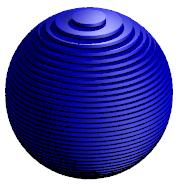
\includegraphics[width=0.2\textwidth]{paste_image3.jpg}
\end{center}

 This is probably confusing, so let us consider finding the volume of a sphere of radius 1 in an interesting way. Suppose we slice up the sphere into small segments of width $\Delta l,$ as shown in the picture above. Instead of $\Delta l,$ we will often call these small segments $dl.$ Note that this isn't divided by anything so it's not a derivative (though it is related to part of a derivative). We'll even integrate over this $dl$ later. Since the segment is small, the volume of the segment is just the area at that location, which I will call $A(l),$ times the width, $\Delta l.$ Since $A(l)$ is just the area of a circle, we know $A(l) = \pi r(l)^2.$ You should convince yourself that you can write $r(l) = \sqrt{1-l^2},$ which seems reasonable as $r(l)$ (or equivalently $A(l))$ should go to zero at the two ends of the sphere. Now, let us add all of these up:

\begin{equation*}
 V \approx \sum \pi(1-l^2) \Delta l
\end{equation*}

 \noindent In the limit that the slices are infinitesimally small, the sum becomes an integral and the result is exact:

\begin{equation*}
 V = \int_{-1}^1 \pi(1-l^2) dl = \frac{4}{3}\pi
\end{equation*}

 \noindent Which is exactly the result you'd expect.



\subsection{Problems}

\begin{center}
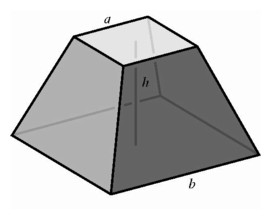
\includegraphics[width=0.3\textwidth]{figure12.jpg}
\end{center}

\begin{enumerate}
 \item There is a truncated square pyramid with dimensions as shown in the figure above. We would like to find the volume of the square pyramid.
 \begin{enumerate}
 \item[a)] Consider taking a small slice with height $\Delta l$ at a position that is nearly a rectangular prism. Write down the volume of this slice. Hint: the volume will depend on your height $l$ 
 \item[b)] Now add up the volume of all these small slices. This is just a Riemann sum and will be an approximation to the volume of the truncated square pyramid.
 \item[c)] Now take the limit that $\Delta l$ is really small and turn your sum into an integral. Evaluate the integral to find the volume of the square pyramid.
 \end{enumerate}
 {\it Note: you can also find the volume by using geometry, but it will be a huge mess!}
 
 \item Suppose we have a tall building like the campanile and we would like to find the total force on it due to gravity. You may think that this should just be the mass of the campanile times the acceleration due to gravity. This isn't quite true, and we'll see how accurate that simple guess is by the end of the problem. For simplicity, assume that the campanile has constant density (mass over volume) $\rho$ and is a rectangular prism with cross-sectional area $A$ and height $H$ (not a very good assumption, but it illustrates the point).

 \begin{enumerate}
 \item[a)] Let's split up the campanile into small slices of height $\Delta h$ with mass $\Delta m$ sitting at a height $h.$ Write down the force on one of these small slices, using Newton's law of universal gravitation.
 \item[b)] Now add up the forces from all the small slices to find a Riemann sum approximation to the total gravitational force on the campanile.
 \item[c)] Take the limit that $\Delta h$ is really small and turn your sum into an integral. Evaluate the integral to find the total force on the campanile.
 \item[d)] How much does your answer differ from the expected result of the total mass of the campanile times the acceleration due to gravity (the campanile is roughly 100~m tall and the radius of the Earth is roughly 6500~km)? Do you care about this difference?
 \item[e)] The campanile obviously does not have constant density and does not have a constant cross-sectional area across its whole height. What would you have to change in this calculation to accommodate these facts?
 \end{enumerate}
\end{enumerate}

\pagebreak

\section{Integrals with Vectors}

{\it See more in Appendix D of your textbook}

\noindent {\it Note: you will probably talk about this more in-depth in Math 53 if you have not taken it yet.}

\noindent First, let's think about integrals that are the dot product of a vector field and a differential such as the integral for work $\int \vec{F}\cdot d\vec{l}.$ In this case, we want to write $d\vec{l}$ such that it points along the path we want to take. This is better explained with a concrete example. Suppose we'd like to calculate $\int \vec{F}\cdot d\vec{l}$ on a path that goes from $(0,0,0)$ to $(1,0,0)$ and then to $(1,1,0).$ Along the first leg, only $x$ is changing, so we can write the differential on this leg as $d\vec{l} = dx \hat{x}.$ Along the second leg, only $y$ is changing, so we can write the differential on this leg as $d\vec{l} = dy \hat{y}.$ Then, the integral becomes:

\begin{equation*}
 \int_0^1 F_x dx+\int_0^1 F_y dy
\end{equation*}

\noindent where $F_x$ and $F_y$ are the $x$ and $y$ components of the force, respectively.

 Now suppose I wanted to take a path from $(0,0,0)$ to $(1,1,0)$ directly along the line that connects the two points. Now, $d\vec{l}$ points in the $\frac{\hat{x}+\hat{y}}{\sqrt{2}}$ direction (the $\sqrt{2}$ is there so that this is still a unit vector). Let me call $dr$ the differential of the position along the line that connects the two points. Then, $d\vec{l} = dr \frac{\hat{x}+\hat{y}}{\sqrt{2}}.$ Now, the integral becomes:

\begin{equation*}
 \int \vec{F}\cdot d\vec{l} = \int_0^{\sqrt{2}} \frac{F_x + F_y}{\sqrt{2}} dr
\end{equation*}

\noindent Here, you would have to write $F_x$ and $F_y$ as functions of $r=\sqrt{x^2+y^2}$ to do this. Alternatively, you could write $dr = \frac{dr}{dx} dx + \frac{dr}{dy} dy$ and do this integral as an integral in $x$ and then as an integral in $y.$

 You can also get an integral in computing the vector field of a quantity. For example, the gravitational force between a point mass $m$ and a mass distribution can be written as:

\begin{equation*}
 \vec{F} = Gm \int \frac{\rho(\vec{r})}{|\vec{r}|^2} \hat{r} dV
\end{equation*}

 \noindent Where $\rho(\vec{r})$ is the mass density at $\vec{r},$ and $\vec{r}$ points from the point mass to a point on the mass distribution (Don't worry too much if you have no clue what this equation means, we'll talk about it later in this course). The important thing that this equation is really {\bf THREE} equations condensed into one. There is an equation here for each component, that is the x,y, and z components of the force (or if you're in cylindrical coordinates, the r,$\theta$, and z components). There are tricks you can do with trigonometry that you will learn later in the course, but the fail-proof way to proceed will be to write $\vec{r} = x \hat{x} + y \hat{y} + z \hat{z},$ and plug this into the equation. Now, I take everything proportional to $\hat{x}$ in the integral of the right hand side, and evaluate the integral (it will turn out you have to write $dV$ in terms of $x,$ $y,$ and $z.$ This will give me the x component of the force. Similarly, if I take everything proportional to $\hat{
y}
$ and $\hat{z},$ I will get the y and z components of the force, respectively.

 A very common mistake is for people to forget that the equation above is really three equations. They think it is just one, and write something like $F = Gm \int \frac{\rho(\vec{r})}{|\vec{r}|^2} dV.$ While this looks similar, it is completely wrong (this will not even give you the magnitude of the force). You really do have to take every component of the force into account.

 \pagebreak
 
\subsection{Problems}

\begin{enumerate}
 \item Suppose a mass feels a force $\vec{F} = -k(\hat{x}+\frac{y}{y_0}\hat{y})$ for some constant $k$ and $y_0.$
 \begin{enumerate}
 \item[a)] What is the work done to get this particle from $(0,0)$ to $(1,y_0)?$ 
 \item[b)] Now, try taking a different path from $(0,0)$ to $(1,y_0)$ and calculate the work again. Is your result different?
\end{enumerate}
\begin{center}
 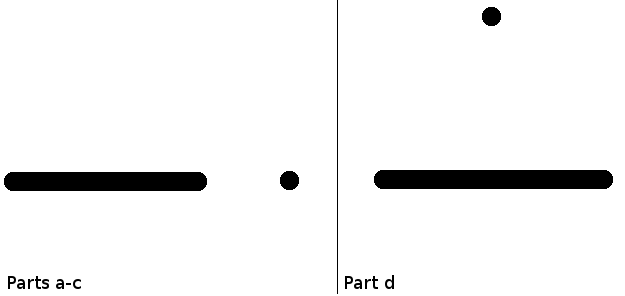
\includegraphics[width=0.5\textwidth]{Rod.png}
\end{center}
\item There is a point mass with mass $m$ a distance $d$ away from a rod with mass $M$ and length $L.$
\begin{enumerate}
 \item[a)] Consider a small portion of the rod $\Delta l$ with mass $\Delta m.$ What is the gravitational force of this small portion on the point mass?
 \item[b)] Add up all the forces from all the small portions of the rod to get an approximation to the total force of the rod on the point mass.
 \item[c)] Take the limit that $\Delta l$ is small and turn the sum into an integral. Evaluate.
 \item[d)] Now suppose the point mass sits on the perpendicular bisector of the rod, a distance $d$ away from the rod. What is the gravitational force of the rod on the point mass now?
\end{enumerate}
 \end{enumerate}

 
 \pagebreak

\section{Probability Distributions}

{\it By Robert Kealhofer and Lenny Evans}

\subsection{The probability density function}

\noindent Suppose we have a distribution of grades of students in a class. Something you may have seen is to put the grades into a histogram, such that the height of a bar on a histogram tells you the number of students that have grades between two values. For example, if the histogram were binned into 5 point intervals, the height of a bar could tell you the number of students that had grades between 90\% and 95\%.  If you wanted to figure out the number of students that had grades between 90\% and 100\%, you would add together the height of the 90-95\% bar and the 95-100\% bar. If the height of each bar is divided by the total number of students, this would give us the probability that a student has a grade in a certain 5 point range. This is the idea behind a probability density function, except instead of binning the students in bins with size 5\%, we bin the students in infinitesimally small bins.

\begin{center}
 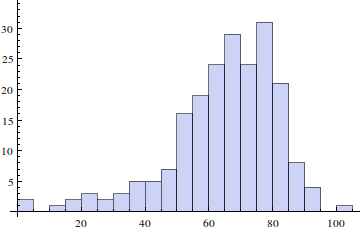
\includegraphics[width=0.45\textwidth]{histogram.png}
\end{center}
Figure 0: A histogram of grades binned in bins of 5\%. \\


The probability density function is a function that you have to integrate to get a probability. In mathematical symbols, suppose that car speeds (or later in this class, gas molecule speeds) are distributed according to some probability density function $f(v)$. If you want to determine the probability that the speed of a car is between $v$ and $v+dv$, you need to write $f(v)dv$. $f(v)$ on its own doesn’t tell you a probability; you must multiply by some interval to get a probability. As a result, because a probability has no units, $f(v)$ has units of inverse velocity so that, when multiplied by a range of speeds $dv$, the result is a unitless probability. {\it Normalization} requires that the probability that the car has a speed between 0 and $\infty$ is 1; that is, $\int_0^\infty f (v)dv = 1$, where the integral runs over all possible values of the speed $v$. This is simply a statement that cars must have {\it some} speed. The probability a car has {\it some} speed (including 0) is 1. Going back to the 
grades example, this is the statement that all students in the course have a grade between 0\% and 100\%. If all the heights of bars of the histogram are added up, it should be equal to the total number of students.

\begin{center}
 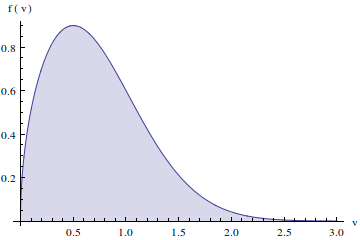
\includegraphics[width=0.45\textwidth]{TotArea.png}
 \end{center}
 Figure 1: $f(v)$ is shown here as a solid line. If $f(v)$ is a probability distribution of the speeds of cars, the total integral under the curve must be 1. This is a statement that a car must have {\it some} speed.
 
 $\\$

Suppose you would like to find the probability that the car’s speed is between two values, $v_1$ and $v_2$ . Recall that the probability that the car’s speed is between values $v$ and $v + dv$ is given by $f(v)dv,$ you simply need to add up (i.e. integrate) all such intervals from $v_1$ to $v_2$ . In symbols, $P(v_1 \leq v \leq v_2 ) = \int_{v_1}^{v_2} f (v)dv$. In a histogram to get the number of students in a certain range that was bigger than the bin size, you had to add up the heights of each of the bins within that range. When the bins become infinitesimally small (and you have a probability distribution), the sum becomes an integral, but the idea is the same.

\begin{center}
 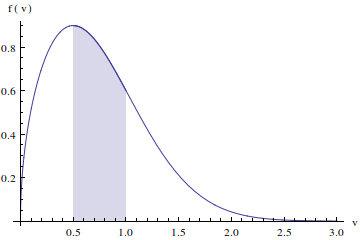
\includegraphics[width=0.45\textwidth]{IntProb.png}
\end{center}
Figure 2: If $f(v),$ shown as a solid line is the distribution of car speeds (say in mph), then the probability that a car has speed between 0.5 and 1 mph is the area under the curve (shaded).


\subsection{Expectation values and averages}

\noindent In physics, we often want to calculate a quantity often called the “expectation value” of a probability density function. The expectation value of a variable $x$ is indicated as $\bar{x}$. The expectation value is basically what you think of as an average (and $\bar{x}$ is probably notation you have used for an average). If you were to have many samples distributed according to some probability distribution function, and then you measured the variable $x$ for each of these samples, the expectation value of $x$ is the average result of all of those measurements. You compute $\bar{x}$ in just the way you are accustomed to computing averages. You take the probability of a particular outcome, and multiply it by the value of $x$ associated with that outcome, and then add them up. In symbols, $\bar{x}= \int x(y) f (y)dy, $where the integral runs over all values of some random variable $y$ of which $x$ is a function. The variable $x$ does not need to be the random variable that the distribution is in 
terms of; it may be a function of that variable. A more concrete example might be the expectation value of vehicle speeds: we would compute $\bar{v}$ as $\int v f (v)dv$, where, once again, the integral runs over all possible values of speed.

The expectation value of a probability density function tells you one thing about the distribution. It tells you where its “center of mass” lies, in some sense, but it doesn’t tell you anything about the shape of the function. For example, two probability density functions might have the same expectation value, but one might look like two lumps on either side of that value and the other might be a single lump at that value. There are other characteristics of probability density functions that we would like to compute.

\subsection{Most probable values}

\noindent One of those characteristics is the most probable value. Suppose I took repeated measurements of some variable $x$, distributed according to some function $f (x)$. $\bar{x}$ would be the weighted average of all of those measurements, but what if I wanted to find the value of $x$ that was most frequent, that is, the most probable value of $x$? I can find that value just as I would find the maximum of any function: by taking the derivative of $f (x)$ with respect to $x$, setting it equal to zero, and solving for $x$. Of course, I would then need to confirm that I found a maximum, either by checking the sign of the second derivative or by knowing something else about $f (x)$.

\begin{center}
 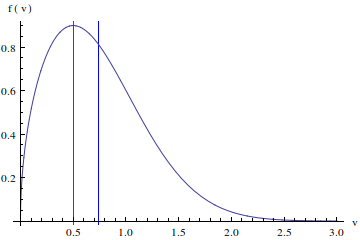
\includegraphics[width=0.5\textwidth]{AvgMax.png}
\end{center}
Figure 3: The most probable value (shown in red) is the maximum of the probability distribution. The average value (shown in blue) can be different from the most probable value.

\subsection{The standard deviation and the variance}

\noindent Another characteristic might be the width of the distribution. Many types of distributions have characteristic widths, and such a width may in fact be defined even if the function does not obviously admit such a definition (e.g. a distribution with multiple lumps). One way to do this might be to get a number by computing the weighted average of how far away values of $x$ are from the expectation value of $x$. Because by definition $\bar{x}$ is at the center of mass of the distribution $f (x)$, it makes sense to add up the squared deviations (i.e. $(x-\bar{x})^2$ ). In this case we define the variance, $\sigma^2$ as $\sigma^2 = \int f (x)(x-\bar{x})^2 dx$. By expanding the square,
it is easy to show that $\sigma^2 =\bar{x^2} - \bar{x}^2$ . Note that those two are not the same thing! For example, $x$ may take on negative values, but $x^2$ does not, so $\bar{x^2}$ will always be larger than (or at worst equal to) $\bar{x}^2.$ The square root of $\bar{x^2}$ is called $x_{rms}$ , the root-mean-square value of $x$.

 We often talk about the standard deviation of $x$, which is the square root of the variance. The standard deviation, qualitatively, tells you how wide the distribution is. A larger standard deviation means that there will be a wider range of possible values for the variable $x$.

\subsection{Summary}

\noindent How do I use a probability distribution function $f (x)$

\begin{itemize}
 \item {\bf to compute a probability? } The probability that the value of the variable $x$ lies between $x_1$ and $x_2$ is given by the integral $\int_{x_1}^{x_2} f(x) dx.$
 \item {\bf to compute an expectation value?} The expectation value of $x$, $\bar{x}$, is computed as $\int x f (x)dx.$
 \item {\bf to compute the most probable value?} The most probable value of $x$ is computed by differentiating $f (x)$ with respect to $x$ and setting the derivative equal to zero. Confirm the value is a maximum with another test.
 \item {\bf to compute the root-mean-square value of $x$?} Compute the square root of the integral $\int x^2 f(x) dx$
 \item {\bf to compute the standard deviation of $x$?} Compute the square root of the difference $\bar{x^2}-\bar{x}^2$

\end{itemize}

\pagebreak

\subsection{Problems}
\begin{enumerate}
 \item Think about how, given a histogram, you would find the average value of the quantity being histogrammed. Can you relate this to the expression for the expectation value of the probability distribution? How about for standard deviation?

 \item Suppose we have a ``continuous die,'' which has a uniform probability of returning any real number between 1 and 6.
 \begin{enumerate}
 \item Plot the probability distribution.
 \item What is the probability of getting $\pi$?
 \item What is the probability of getting a number between 3 and 4?
 \item What is the most probable value that the die will give?
 \item What is the average value that the die will give?
 \item Suppose I get many numbers from this continuous die. What will be the standard deviation of these numbers?
 \item Suppose I get many numbers from this continuous die. What would I expect the average of the exponential of these numbers to be?
 \end{enumerate}
\end{enumerate}


\pagebreak

\section{Dimensional Analysis}
{\it See more in Appendix C of your textbook}


\noindent {\it In this section we will use the notation [A] to mean the units of A.}

\noindent Let F and G denote arbitrary physical quantities. An equation in physics of the form F = G, can not be true if [F] $\neq$ [G].

 Similarly, addition and subtraction operations of the form F $\pm$ G, are meaningless if [F ] $\neq$ [G].

 Note that multiplication and division can be done between F and G even if they have different units.

One good check to do if your answer has a function is to see if the argument of the function is unitless. The statement $\sin(1~\mathrm{second})$ does not have a meaning, so if you get something like $\sin(T)$ where $T$ is a time as your answer, you have probably done something wrong. Similar things can be said about $\cos(x),$ $\ln(x),$ and raising numbers to powers, such as $e^x.$ Note that the output of a function will also be unitless. $\cos(5)$ is just a number, it does not contribute any units.

 Many of the equations in E+M have units that are annoying to figure out. Most of your GSIs would probably have to think for a bit about how to relate henries and farads to joules. However, knowing these relations is not necessary to be able to check your units. Take for example Newton's law of universal gravitation, $\vec{F} = \frac{G m_1 m_2}{|\vec{r}|^2}\hat{r}.$ $G$ has some weird units that are hard to remember, but a good check in your final answer would be to see if your force has $G$ multiplying 2 masses and divided by 2 length scales. It's often easier to compare to a basic equation like this than to try to figure out what the units of each thing actually are.

 \pagebreak

\subsection{Problems}
In the following problems $G$ is Newton's constant, $a$ and $r$ are lengths and $M$ and $m$ are masses.
\begin{enumerate}
 \item Why is $\vec{F}(r) = \frac{GMma}{(a+r)^3}\hat{r}$ a valid gravitational force, but $\vec{F}(r) = \frac{GMm}{(a+r)^3}\hat{r}$ not?
 \item Suppose I determine that the energy of a gravitational system is $G\rho^2 a^5$ where $\rho$ is a mass density (mass/volume). Should I be worried about my answer?
 \item Suppose I determine that a distance of closest approach for some system is $\frac{G M m}{5 m v^2-v^2},$ where $v$ is a velocity. Should I be worried about my answer?
\end{enumerate}

\chapter{Temperature and Kinetic Theory}

\section{Chapter 17}

You may want to review section 0.1 before attempting the problems in this section.

\subsection{Problems}
\begin{enumerate}
 \item You have a cylinder that has a length $L$ and a radius $R.$ The thermal expansion of this cylinder is anisotropic. Its length expands with linear expansion coefficient $\alpha_L$ and its radial dimension expands with linear expansion coefficient $\alpha_R.$ What is the volume expansion coefficient of the cylinder?
 \item Suppose we have a box of volume $V$ divided into two equal volumes $V$/2 with gas at some pressure $P$ on one side and a vacuum ($P = 0$) on the other side.
 \begin{enumerate}                                                                                                                                                                                                       
 \item We slowly move the partition over so that the side containing the gas now fills the full volume $V$.
 \item What happens to the temperature and pressure of the gas?
 \item Can we explain this in terms of the kinematics of the molecules bouncing off walls?
 \item Does this give us some mechanism to reduce the average speed of the molecules?
\end{enumerate}                                                                                                                                                            \end{enumerate}

\pagebreak
                                                                                                                                                                                                              
                                                                                                                                                                                                              \section{Chapter 18}                                                                                                                                                                                                            {\it For a simple derivation of the Maxwell speed distribution, please see the appendix}

You may want to review section 0.4 before attempting the problems in this section and the workbook. Note that section 0.4 talks about probability distributions. To make a speed distribution (as defined in the book) a probability distribution you divide by the total number of particles (if this doesn't make sense, make sure to ask why this is!). Understanding this section can be tricky, so be sure to ask your GSI lots of questions if you are confused!                                                                                                                                                                                         
                                                                                                                                                                                                              
\subsection{Problems}

\begin{enumerate}
 \item In this problem we will determine the relationship between kinetic energy and temperature for a gas that lives in a 2D world. Consider molecules with mass $m$ that bounce elastically with velocity $\vec{v}$ inside a square of area $L^2.$

\begin{enumerate}
 \item Consider one wall of the container. What is the average time per molecular collision with that wall?
 \item What is the average change in momentum of a molecule per collision, $\Delta \vec{p}$?
 \item What is the average pressure $P$ (force per unit length of wall) on the wall?
 \item If the ideal gas law in two dimensions is $PA = NkT,$ what is the relationship between kinetic energy and temperature?
\end{enumerate}
                                                                                                                                                                                  \item Suppose that the speed distribution of a collection of $N$ gas molecules is $f(v) = A v^2$ for some constant $A$ if $v<v_0$ and 0 otherwise.
\begin{enumerate}
\item Make a plot of the probability distribution.
\item Determine the value of the constant $A$
\item Determine $\bar{v}.$
\item Determine $v_p,$ the most probable speed. Does taking a derivative of the distribution help you find this? What is the probability of measuring the speed and obtaining $v_p$?
\item Determine $v_{rms}$.
\item What is the standard deviation of the speed of these gas molecules?
\end{enumerate}
\item Suppose you are riding on a train that has a velocity $v$. You see out of the window a clear box
with an ideal gas. You happen to be wearing special goggles that allow you to see the distribution
of molecular speeds in the box. If you were to calculate the temperature of the box from your
observation would it be higher than the temperature measured from someone not on the train? Justify your
answer on physical grounds.

\pagebreak
\item Draw three different speed distributions that have the same:
\begin{enumerate}
\item temperature
\item rms velocity
\item most probable velocity
\item average speed
\end{enumerate}
\end{enumerate}

\chapter{First Law of Thermodynamics}

\section{Chapter 19}

You may want to review section 0.2 before attempting some of the problems in this section. There are a few relationships in this section (such as equations for $Q$), that are only applicable in certain scenarios. Make sure you get straight which equations are always applicable (such as the first law of thermodynamics) and which ones hold only under certain assumptions.


\subsection{Problems}
\begin{enumerate}
 \item Suppose the specific heat of a material is given by $c(T) = k \frac{T}{T_0}.$ How much heat is required to change a mass $m$ of that material from a temperature $T_1$ to $T_2$?
 \item Use the first law of thermodynamics to show that $C_V = C_P+R.$
 \item Use the equipartition theorem and the first law of thermodynamics for a constant volume process to show that $C_V = \frac{d}{2} R.$
 \item Does adding heat to a system always increase the temperature? Why or why not?
\item The Van der Waals Equation of state is an alternative, more realistic, model for gases than the ideal gas law (you just need the formula for this problem). It has two extra constants $a$ and $b$ such that $(P+\frac{a}{(V/n)^2})(\frac{V}{n}-b) = RT.$ Calculate the work done in an isothermal expansion of a Van der Waals gas from $P_1, V_1$ to $P_2, V_2.$
\item Consider $N$ particles of an ideal gas undergoing a thermodynamic process going from a temperature $T_0$ and volume $V_0$ to a temperature $T_f$ and volume $V_f.$ Along this thermodynamic process, the relation $\frac{T}{V^2}=$const. holds.
\begin{enumerate}
 \item Calculate the work done, change in internal energy, and the heat change as the gas underwent this process.
 \item What does this process look like on a PV diagram, and how does it compare to the four processes you have learned about in class? 
\end{enumerate}
 \item Consider a gas in a closed container that is pushed to a smaller space with a piston. An adiabatic process is one in which the work-energy theorem holds for the gas; even though we had to push on the piston to push in the gas to do work on it, all of the work went straight to the gas and wasn’t lost in the random motion of particles in the piston.
 \begin{enumerate}
  \item Show that in this scenario $PV = (\gamma-1)U.$
  \item Differentiate this equation with respect to volume. Do not assume $P$ is a constant, or that you know how $P$ changes with $V$ (I never said it had to be constant temperature or anything). Therefore you’ll need to have $dP/dV$ in your solution.
  \item Multiply your solution to (b) by $dV$. Use the first law of thermodynamics and the fact that there is no heat added in adiabatic process to solve for $P$ as a function of $V$. This is the adiabatic formula that you learned in class.
 \end{enumerate}


 \item There are $N$ molecules of an ideal gas with $n$ degrees of freedom. This gas undergoes an adiabatic process starting at a pressure $P_0$ and $V_0.$
 \begin{enumerate}
 \item When the volume of the gas is $V_1,$ what is the temperature of the gas?
 \item Suppose the this temperature is changed by a small amount $dT.$ How does this change the volume? Call this volume change $dV.$
 \item The thermal expansion coefficient is the change in volume you get when you change the temperature of the gas a small amount. What is the thermal expansion coefficient of the gas when the volume is $V_1?$
 \item Why is the thermal expansion coefficient you got negative?
 \end{enumerate}
  \item You have two materials with thermal conductivities $k_1,$ and $k_2.$
 \begin{enumerate}
  \item What is the effective thermal conductivity if the materials are in series?
  \item What is the effective thermal conductivity if the materials are in parallel?
  \item Make qualitative plots of the temperature in the materials if one end is in contact with a hot temperature and the other end with a cold temperature.
  \end{enumerate}
 \item While Einstein believed the universe was unchanging in volume, more recent experimental evidence suggests that the universe is actually getting larger. The universe expands adiabatically, because no heat can flow. Estimate the temperature of the universe when the universe was 2~cm in diameter, compared to the current temperature of 3~K. Assume that the non-hydrogen gas parts of the universe can be neglected.
 \item Suppose we have a thermal process for an ideal gas where $dQ = \frac{1}{2} dE.$ In this process, it is true that $PV^\beta=$const., for some $\beta.$ What is the value of $\beta?$
 \item Why does a bike pump get hot when you are inflating bike tires? Can we treat this as an adiabatic process and if so, why? Explain this in terms of a P-V diagram.
 \item Consider a wire of length $L$ and whose radius varies linearly from one end to the other. One end has
radius $r_A$ and temperature $T_A$ while the other end has radius $r_B$ and temperature $T_B$ . The thermal
conductivity is $K$.
\begin{enumerate}
 \item Find the rate of heat flow through the wire.
 \item Make a qualitative plot of the temperature as a function of position along the wire.
 \item Assume that $r_B$ = $2r_A$, find the temperature at a point half-way
down the wire, at $L/2$.
\end{enumerate}
 \item We will consider the radiation balance between the earth and the sun, assumed to be both
perfect black body radiators at constant temperature.
\begin{enumerate}
 \item We assume first that there are no greenhouse gases in the atmosphere.
Knowing the radius of the sun ($R_S=7\times 10^8$~m), the mean earth-sun distance ($D_{SE}=
1.50\times 10^{11}$~m) and the temperature of the sun ($T_S=5800$~K) compute the mean
temperature $T_E$ of the earth.
\item We now introduce a greenhouse gas layer, very close to the surface of
the earth. We will assume that the greenhouse layer does not absorb the (mainly
visible) solar radiation but fully absorbs (and reemits over the $4\pi$ solid angle) the
(infrared) radiation reemitted by the earth. By writing down the energy flux
balance for the greenhouse layer and the earth separately, compute the new
temperature of the earth. The greenhouse layer emits both inside and outside.
\end{enumerate}
\end{enumerate}

\chapter{Second Law of Thermodynamics}

\section{Chapter 20}

The entropy relation given in your book only applies to reversible processes. If you have an ideal gas, you can calculate entropy change in a non-reversible process by using the fact entropy is a state variable. You can connect the two ends of the non-reversible process with a sequence of reversible processes. For non-gases, you can often consider a non-reversible process as a sequence of reversible processes and calculate entropy change this way.

\subsection{Problems}

\begin{enumerate}
 \item To help the “energy crisis” a group of physicists decide to use a geothermal area to operate a heat engine
to produce electricity. They discover a 30 $km^3$ region of hot rock underground with a temperature of
$T_o = 600^{\circ}$C. Water is pumped into the rock and the emerging steam used to run the electric generator.
This may be thought of as a heat engine whose ambient exhaust temperature is the atmosphere ($T_a =
20^{\circ}$C). As the rock cools the rate of steam production decreases and the physicists plan to quit the project
when the rock temperature has dropped to $T_f = 110^{\circ}$C. Find the maximum amount of electrical energy
(in kWhr) that can be generated. The rock’s density is $\rho = 7000 $kgm$^{-3}$ and the rock’s specific heat is
$c = 103$ J/kg·K.
\item A gas is at pressure $P_0$ and and volume $V_0.$ With the volume held constant, the pressure is now doubled. Then, with the pressure is held constant and the volume is now doubled. Each of these steps is then repeated 9 more times. What is the total change in entropy after all of the steps?
\end{enumerate}


\chapter{Electric Charge and Electric Field}

\section{Chapter 21}

You may want to look over section 0.2 and 0.3 before trying the problems in this section. In fact, the problems in section 0.2 could have been problems in this section if the symbols were changed around.

Remember, electric field is a {\it vector!} That means you need to describe each of its components when you are asked to find it. Also, note that because electric field is a vector, Coulomb's law is really a set of three equations. Often you can argue that a few of these equations should be trivial, but you should recognize that the equations are always there.

\subsection{Problems}

\begin{enumerate}
 \item There is an electric field over all space that looks like $\vec{E} = \alpha(x \hat{x} - y^2 \hat{y}).$ There is a rod of length $L$ with charge $Q$ distributed uniformly across it. What is the force on the rod if one end of the rod is at $(0,0)$ and the other end at:
 \begin{enumerate}
  \item $(0,L)?$
  \item $(L,0)?$
  \item $(\frac{L}{\sqrt{2}},\frac{L}{\sqrt{2}})?$
 \end{enumerate}
 
 \pagebreak
 
 
\begin{center}
\begin{figure}[h]
\centering
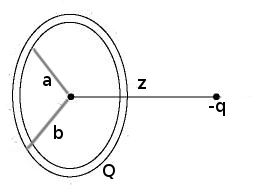
\includegraphics[width=150px]{Prelab2Pic.jpeg}
\end{figure}
\end{center}

 \item There is a ring with inner radius $a$ and outer radius $b$ that is uniformly charged with a charge $Q>0.$ A point charge $-q$ (with $q>0$) sits a distance $z$ (perpendicular to the plane of the ring) above the center of the ring.
 
 \begin{enumerate}
 \item Find the force on the point charge.
 \item Now suppose the point charge is very close to the ring. Find the frequency of oscillation of the point charge. How close does the point charge need to be for this to be valid?
 \item How does the force on the point charge depend on $z$ if $z$ is large? Why is it reasonable to expect the force to look like this when $z$ is large? How far does the point charge need to be for this to be valid?
 \end{enumerate}
 
\begin{center}
 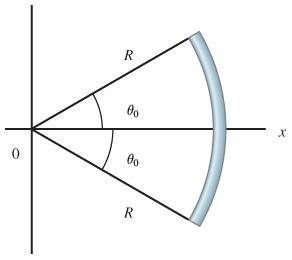
\includegraphics[width=150px]{jlkj.jpg}
\end{center}
 
 \item A thin rod bent into the shape  of an  arc of a circle of radius $R$ carries a uniform charge
per  unit length  $\lambda>0.$  The arc  subtends  a total  angle  $2\theta_0$, symmetric about the $x$- axis, as shown above.
 \begin{enumerate}
 \item Determine the magnitude and direction of the electric field at the origin.
 \item When $\theta_0\to 0,$   but  the total charge, $Q$, remains constant what does the field look like. Why would you expect the field to have this form?
 \end{enumerate}

 \pagebreak
 
 \item A thin, ring-shaped wire of radius $R$ holds a total charge $+Q$ distributed around it.
 
  \begin{enumerate}
 \item Determine the electric field on its symmetry axis, a distance $x$ from the center of the ring.
 \item Now suppose you have two of these rings, both with charge $+Q,$ separated by a distance $R$ (sharing the same symmetry axis). How does the electric field scale with $x$ very close to the midpoint of the two rings? How does the electric field scale with $x$ far away from the two rings? Explain why you should expect the field to look like this far way.
 \item Now suppose that one of the rings (say the left one) has charge $-Q$ and the other has charge $+Q.$ How does the electric field scale with $x$ very close to the midpoint of the two rings? How does the electric field scale with $x$ far away from the two rings? Explain why you should expect the field to look like this far away.
 \item Now suppose you have four of these rings, arranged in a line sharing the same symmetry axis. Each ring is separated by a distance $a$ from the nearest ring. You would like to make an electric field centered at a position $x_0$ in between the rings. You would like this to be as close to quadratic as possible, with the coefficient of the quadratic term being $\alpha.$ What should the charges be on each of the rings?
 \end{enumerate}
 
 \item You have two rods of length $L$ with charge $Q$ uniformly distributed on them. The rods are colinear and the centers are separated by a distance $d.$

 \begin{enumerate}
\item What is the force one rod exerts on the other?
\item When the two rods are separated by a large distance (that is, when $d\gg L$), how does the force scale with $d?$ Why would you expect it to look like this?
 \end{enumerate}
 
 \item Consider a hemispherical shell of surface charge density $\sigma$. Find the electric field on the symmetry axis of the shell at an arbitrary height.
 
\end{enumerate}

\chapter{Electric Flux and Gauss's Law}

\section{Chapter 22}

While Gauss's law problems tend to be simple, you should be fully aware of when it is useful and when it is not. You would like the normal vector to a Gaussian surface to either be parallel or perpendicular to the direction of the electric field, and the electric field should be constant over the surface. This is the only way that $\oint \vec{E}\cdot d\vec{A}$ becomes $|\vec{E}| A$ or 0 depending on the direction of the electric field.

This may sound like a tricky set of rules. In practice, the only examples where Gauss's law is useful to find the electric field are given in the textbook. This includes spheres of charge (and point charges), infinite cylinders of charge (and infinite lines of charge), and infinite slabs of charge (and infinite sheets of charge). Note that Gauss's law can be used to find the approximate field for very long cylinders and large slabs as long as one desires to find the field far away from the edges.

A good rule of thumb is to use Gauss's law if you see any of these geometries. It will certainly be easier than using Coulomb's law (though it is still possible to use Coulomb's law). If there is any other geometry, Coulomb's law must be used.

When you use Gauss's law, you must be explicit about what Gaussian surface you are using. If you are turning in a problem, you should not assume that the grader assumes that you know what Gaussian surface you have chosen. Even in the scenarios described above, Gauss's law is useless if you choose a bad Gaussian surface. For example, if you have a plane of charge and use a spherical Gaussian surface, you cannot determine the electric field.

\pagebreak

\subsection{Problems}

\begin{center}
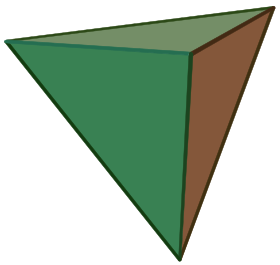
\includegraphics[width=0.15\textwidth]{Tetrahedron.png}
\end{center}
\begin{enumerate}
 \item A point charge with charge $Q$ lies at the center of a face of a regular tetrahedron. What is the electric flux through any of the other faces?
 \begin{center}
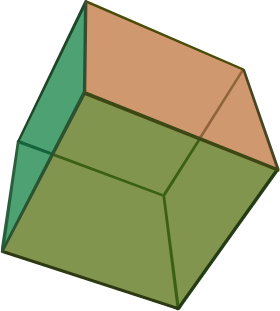
\includegraphics[width=0.15\textwidth]{Hexahedron.png}
\end{center}
 \item A point charge with charge $Q$ is at the corner of a regular hexahedron (more commonly known as a cube). What is the electric flux through a face that does not contain that corner?
 \item Write down Gauss's law for gravitational fields. Can the gravitational flux be negative? Can it be positive?
\end{enumerate}


\chapter{Electric Potential}

\section{Chapter 23}

The potential is related to the integral of the electric field. Integrals tend to ``smooth'' out functions. This means that while electric fields may have discontinuities, the electric potential is always continuous!

Note that to use the equation $V = -\int \vec{E} \cdot d\vec{l},$ it is necessary to choose a path along which to integrate. This path is not obvious, so if you are turning in a problem you should be explicit about what path you have chosen.

Note that to use the equation $\vec{E} = -\vec{\nabla} V,$ it does not suffice to know the potential at just one point. This equation says that electric field is some kind of derivative of $V,$ and if you think back to the definition of a derivative ($\frac{df}{dx} = \displaystyle\lim_{h\to0} \frac{f(x+h)-f(x)}{h}$), you have to know the potential at a position $x$ AND $x+h$ to be able to find the derivative. Thus, you need to know the potential at a series of points.

If you are asked to find electric field and potential, there are a few strategies to take. In general, taking a derivative is easier than taking an integral, so it is often easier to use Coulomb's law with potential and then take a derivative, than to use Coulomb's law with electric field and take an integral (and both options are most likely easier than using Coulomb's law to find both). Even if you are just asked to find the electric field, the potential equations are simpler so you may make fewer mistakes calculating potential to find the electric field. However, there is no Gauss's law analogue for potential. Since using Gauss's law is easier than using Coulomb's law, if there is a scenario where Gauss's law is applicable, it is often easier to find the electric field using Gauss's law and then integrating to find the potential. 

\pagebreak

\subsection{Problems}

\begin{enumerate}
 
 \item There is a point charge $-q$ sitting in the center of a hollow conducting sphere with inner radius $a$ and outer radius $b.$
 \begin{enumerate}
 \item How does the charge distribute itself on the conductor? Why does this happen?
 \item Make qualitative plots of what you would expect the electric field and potential to look like.
 \item Now calculate the electric field and the potential. Does it agree with your expectations?
 \end{enumerate}
 \item There is a sphere of radius $R$ with charge $Q$ on it.
 \begin{enumerate}
  \item Calculate the self energy of the charge distribution if the charge is uniformly distributed.
  \item Calculate the self energy of the charge distribution if all the charge is on the outer surface of the sphere.
  \item Use these results to explain why charges arrange themselves in the way they do in conductors. Can you prove that this is the most optimal thing for a conductor to do?
 \end{enumerate}

\end{enumerate}

\chapter{Capacitance}

A common mistake that is made when calculating the electric field of a capacitor plate (in order to find the potential) is to choose the wrong Gaussian surface. For example, in a parallel plate capacitor, this would be choosing a Gaussian surface that encompasses the whole plate. As I hope you have learned a few chapters ago, this is not a regime where Gauss's law is valid. Instead, we are making the assumption that the plate is very large, and are finding the field far from the edges. The Gaussian surface should be much smaller than the one described before.

Note that capacitors have a physical space between the two plates. Unless the capacitor is not working properly, this means that no charge can travel from one plate to the other. Thus, if there are plates of the capacitor that are not connected to a charge source (such as a battery), there is no way that the plates can acquire any net charge. Note this does not mean that any individual plate in the configuration cannot acquire charge, but the total charge of all the plates must be zero.

\begin{center}
\begin{circuitikz} \draw
(0,0) to[battery] (0,2)
      to[C] (2,2)
      to[C] (2,0) --(0,0)
;\end{circuitikz}
\end{center}


For example, in the circuit above, the two plates touching the upper right corner are isolated (by space) from the battery. Since there is no charge in this region before the battery is hooked up, this means that no charge can be there when the battery is hooked up. This means that the charges on these two capacitor plates must be equal and opposite. 

\pagebreak

\section{Chapter 24}

\subsection{Problems}

\begin{enumerate}
\item Let's suppose the electron were a sphere of uniformly distributed charge. Relate the self-energy of the electron to the mass using $E=mc^2,$ where $c = 3\times10^{8}$~m/s is the speed of light. In this model what is the radius of the electron? Note that Penning trap measurements show that the radius of the electron should be smaller than $10^{-22}$~m.
 \item A cylindrical capacitor (with inner radius $a$ and outer radius $b$) is placed in a tank of dielectric oil. The oil has a dielectric constant $\kappa$ and a mass density $\rho$. If the potential of the inner cylinder is held constant at $V$ and the outer cylinder is at zero potential, then to what height, $h$, will the oil rise within in the cylinders?
 
  \begin{center}
  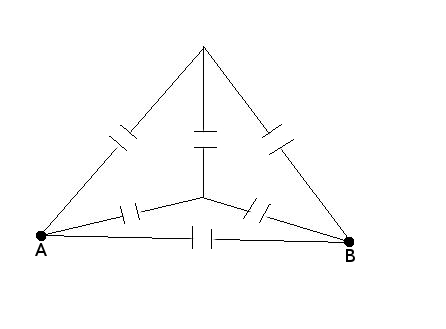
\includegraphics[width=150px]{Tetrahedron.JPG}
 \end{center}
 
 \item 6 capacitors with capacitance $C$ are arranged in a tetrahedron, as shown above.
 \begin{enumerate}
  \item Can you use series/parallel rules to simplify this circuit? Why or why not?
  \item Write down the charge conservation equations for the arrangement. Can you manipulate them to determine anything interesting?
  \item A battery is hooked up to the A and B terminals. Considering the voltage drop across the capacitors, write down enough equations to be able to solve for all the charges on all 6 capacitors.
  \item Do you see how you might be able to simplify all of these equations?
  \item What is the equivalent capacitance of the system?
 \end{enumerate}
 
 \pagebreak
 
  \begin{center}
  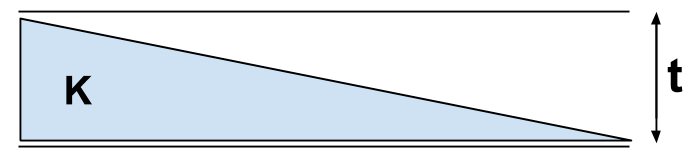
\includegraphics[width=150px]{CapacitorDrawing.png}
 \end{center}

 
 \item A parallel plate capacitor has a capacitance $C$ when there is no dielectric inside of it. Suppose a wedge of material with dielectric constant $K$ is inserted in between the plates of the capacitor (see figure). The bottom face of the wedge has the same area as the plate of the capacitor. The height of the wedge is equal to the thickness of the capacitor, $t$ on the left edge and varies linearly until the height is zero on the right edge. What is the new capacitance with this dielectric inserted?
 
 \begin{center}
  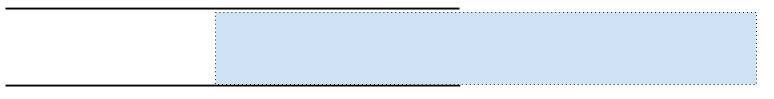
\includegraphics[width=200px]{CapProb.png}
 \end{center}

 
 \item A slab of width $d$ and dielectric constant $K$ is inserted a distance $x$ into the space between the square parallel plates (of side length $L$) of a capacitor. 
 
 \begin{enumerate}
  \item Suppose this capacitor is hooked up to a battery with voltage $V.$ What is the force on the dielectric?
  \item Suppose the capacitor is fully charged, but not connected to the battery. What is the force on the dielectric?
 \end{enumerate}
 
 \item  Consider two parallel, infinitely long conductive wires, each with radius $a,$ one with linear charge density $\lambda,$ and the other with linear charge density $-\lambda.$
 
 \begin{enumerate}
 \item  Find the electric field between the wires (don't worry about the rest of space) as a function of $r,$ the distance from the center of one wire.
 \item  Find the potential difference between the wires. Why do we not need to worry about the
potential going to infinity like we did with infinitely long lines of charge?
\item Find the capacitance of the system.
 \end{enumerate}
 
 \end{enumerate}


\chapter{Resistance and Ohm's Law}

\section{Chapter 25}

\subsection{Problems}
\begin{enumerate}
 \item You would like to build a voltmeter. How should it connect to the circuit, and how should it measure the voltage? Should it have a large resistance or a small resistance?
 \item You would like to build an ammeter (a device that measures current). How should it connect to the circuit? Should it have a large resistance or a small resistance?
  \item Suppose you have a cylindrical resistor with radius $R$ and length $L.$ Suppose the resistor has a thermal volume expansion coefficient of $\beta.$ Assuming that the resistivity of the material the resistor is made of has no temperature dependence, what is the change in resistance due to thermal expansion?
  \begin{center}
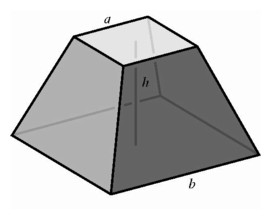
\includegraphics[width=0.3\textwidth]{figure12.jpg}
\end{center}

 \item There is a truncated square pyramidal resistor with dimensions as shown in the figure above. If the material is made of material with resistivity $\rho,$ what is its resistance? (If it bothers you that the current may not distribute itself evenly, you can assume $b-a\ll h$).
 
 \pagebreak
 
 \item A resistor is made from two concentric spheres with radii $a$ and $b$ between which there is a material with resistivity that varies with radius as $\rho(r) = \rho_0 \left(\frac{r}{a}\right)^s,$ where $\rho_0$ is a constant. A battery with voltage $V$ is hooked up to the resistor such that current is injected into the resistor from the inner sphere, and removed from the outer sphere.
\begin{enumerate}
 \item What must the exponent, $s,$ be if the electric field between the spheres is constant?
 \item What is the current, $I$ in the circuit?
\end{enumerate}

\end{enumerate}

\chapter{DC Circuits}

When faced with a circuit, what you should do is use Kirchoff's rules to write down a system of equations. Then, you can use algebra to solve the system. If it is an RC circuit, you will want to get an equation that has both $\frac{dQ}{dt}$ and $Q,$ so that you will have a differential equation you can solve.

\section{Chapter 26}

\subsection{Problems}
\begin{enumerate}
 \item You would like to design a capacitive screen for a cell phone. What kind of circuit might you build? Estimate values you could choose for the circuit components.
 \item You would like to design a control system for windshield wipers. What kind of circuit might you build? Estimate values you could choose for the circuit components.
 \item When building a circuit, why might you want to avoid having wires make sharp turns?
 \item Why are series/parallel rules for batteries not shown in the book?
  \item You have a 2D grid of resistors infinite in extent (like graph paper). Each resistor has resistance $R.$ What is the equivalent resistance between two adjacent nodes? Can you extend your result to the case where you have an $n$-dimensional grid, for any value of $n$?
  
  \pagebreak
  
  \begin{center}
  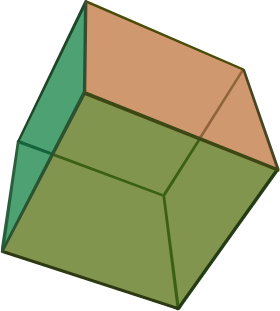
\includegraphics[width=0.15\textwidth]{Hexahedron.png}
\end{center}
 \item You have resistors of resistance $R$ along each edge of a regular hexahedron (more commonly known as a cube). What is the equivalent resistance between one corner and the corner furthest from it?
 \begin{center}
\begin{circuitikz}\draw
(0,0) to (0,1)
to [R=$R$] (4,1)
to (4,0)
(0,0) to [R=$R$] (2,0)
to [R=$R$] (4,0)
to [R=$R$] (6,0)
(2,0) to (2,-1)
to [R=$R$] (6,-1)
to (6,0)
(0,0) to (0,-2)
to [battery] (6,-2)
to (6,-1)

;\end{circuitikz}
\end{center}
 \item Find the equivalent resistance of the network of resistors shown above.
\item Consider the following circuit:
\begin{center}
\begin{circuitikz}\draw
(0,0) to [battery](0,2)
to [cspst] (2,2)
to [R](2,0)
to (0,0)
(2,2)  to [C] (4,2)
to [R] (4,-2)
to [C] (2,0)
(4,-2) to (0,-2)
to [R] (0,0)
;\end{circuitikz}
\end{center}
The capacitors are initially uncharged and the switch is closed at $t=0.$ If the resistors have resistance $R$ and the capacitors capacitance $C,$ what is the current through the diagonal capacitor?

\pagebreak

\item An initially uncharged capacitor with capacitance $C$ is connected to two resistors of resistance $R$ and a battery with voltage $V$ in the arrangement below:

\begin{center}
 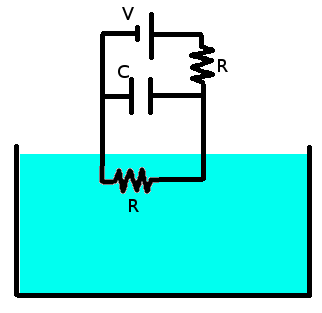
\includegraphics[width=0.3\textwidth]{Prelab5S22014.png}
\end{center}


\noindent The resistor in parallel to the capacitor is immersed in a vat of water as all the components are connected. There is a mass $m$ of water (with specific heat $c_w$) and it is initially at a temperature $T_0.$ You may assume that $m$ is sufficiently large and $T_0$ is sufficiently far from the boiling point or freezing point of water such that there is no phase change that occurs. What is the temperature of the water as a function of time? What assumptions did you have to make to make this problem tractable?


\end{enumerate}

\chapter{Magnetism}

You may notice that Ampere's law looks kind of like Gauss's law. Just as with Gauss's law, where there were only a few scenarios where Gauss's law is useful, there are only a few scenarios where Ampere's law is useful. These are solenoids, toroids, infinite cylinders (and wires), and infinite slabs (and sheets).

Biot-Savart law is actually very similar to Coulomb's law. You set the problems up almost exactly the same way. The only complication here is the cross-product. One way to do this is to write $d\vec{l}$ and $\hat{r}$ in vector form and then take the cross-product using the rules you know about taking cross products. Others find it fruitful to interpret this as $dl \sin(\theta),$ and properly interpret $\theta$ and the direction the $\vec{B}$ field should point. Either way you do it will work, but make sure you get practice. As with Coulomb's law, Biot-Savart law is really a collection of three equations. Often some of these equations will be trivial, but it is important to realize that there are always three equations.

\section{Chapter 27}

\subsection{Problems}
\begin{enumerate}
\item There is a point in space where you would like to measure the electric and magnetic fields. You can measure the force vector (three components) on particles at that point. How many particles do you have to measure the force on to fully determine the electric and magnetic fields?
 \item In a region of space, there is a magnetic field $\vec{B} = \beta( x \hat{x} - z \hat{z}).$ A wire of length $L$ carries a current $I.$ One end of the wire is at the origin, and the wire makes an angle $\theta$ with the $x$ axis, in the $x-y$ plane. What is the force on the wire?
 \item Using the force equation $\vec{F} = q \vec{v}\times\vec{B},$ show that magnetic fields do no work.
 \item Can the magnetic field be written as the gradient of a potential (that is, $\vec{B} = -\vec{\nabla}V$) like electric field? There are actually cases when you can and cannot, so try to figure out when these cases are.
 \item Explain how the Hall effect can be used to differentiate the sign of the mobile charges in a material. Derive the Hall voltage for a material with dimensions $w, l, h$
in a uniform magnetic field $B = B_0 \hat{z}$ with total current $I.$

\end{enumerate}

\pagebreak


\section{Chapter 28}

\subsection{Problems}
\begin{enumerate}
\item There in a region of free space (somewhere where there are no wires), which may have current carrying wires outside of the region.
\begin{enumerate}
\item Is it possible to construct a maximum of magnetic field magnitude?
\item How about a minimum of magnetic field magnitude?
\item Suppose you have atoms with magnetic moment $\vec{\mu}.$ What are the conditions to trap these atoms somewhere in this region of free space?
\end{enumerate}

\item There is a long wire with radius $R.$ A hole of radius $R/2$ is cut out of the wire, centered at a position $R/2$ away from the center. If a current $I$ flows through the wire with the hole cut out, what is the magnetic field everywhere?
  \item In this problem we will think about the magnetic field created by Helmholtz coils. You will be using these in the magnetism lab. You have a circular loop of radius $a$ with a current $I$ flowing through it.
  \begin{enumerate}
   \item Find the magnetic field at any point on the axis of symmetry of the loop.
   \item Now suppose you have two of these loops, separated by a distance $a.$ What is the magnetic field at the center of the loops?
   \item Suppose you are now a small distance $x\ll a$ away from the center (along the axis of symmetry). What does the magnetic field look like at this location?
   \item Now suppose you have two of these loops, but the currents are flowing in opposite directions. When you are a small distance $x$ away from the center (along the axis of symmetry) what does the magnetic field look like at this location?
  \end{enumerate}
  \item We would like to find the magnetic field due to a sheet of current with width $w$, carrying current per unit length $K$. The sheet extends infinitely in the direction perpendicular to the width.
  \begin{enumerate}
  \item Can you use Ampere's law to solve this problem? Why or why not?
  \item As a preliminary, using Biot-Savart law, determine the magnetic field from a wire caring a current $I.$
  \item Use the result from part a) to find the magnetic field of the whole sheet. Note that you can write $K = \frac{dI}{dx}.$
  \item Now take the limit as $w\to\infty.$ Use Ampere's law to verify that what you get is correct.
  \end{enumerate}
  
  \pagebreak
  
  \item You have a rod of length $L$ with charge $Q$ distributed uniformly across it. This rod spins about one of its ends with angular frequency $\omega.$
  \begin{enumerate}
  \item What is the magnetic dipole moment of the rotating rod?
  \item What is the magnetic field due to the rotating rod?
  \item Does your result agree with what you would expect for the field due to a magnetic dipole moment?
  \end{enumerate}
  \item A nonconducting circular disk, of radius $R$ and negligible thickness, carries a uniformly distributed electric charge $Q$. The plate is set spinning with angular velocity $\omega$ about an axis perpendicular to the plate through its center.
  \begin{enumerate}
  \item Determine the magnetic field at points on its rotation axis a distance $x$ from its center.
  \item Now suppose you have a sphere with radius $R$ carrying a uniformly distributed electric charge $Q,$ spinning at an angular velocity $\omega.$ Use the previous result to calculate the magnetic field at points on its rotation axis, a distance $x>R$ from its center.
  \item What is the leading asymptotic behavior far away from the sphere? How could you have obtained this more easily?
  \end{enumerate}
  \item  A semicircular wire carries current $I$. Let the current lie on a circle of radius $a$ with $\theta$ from $\pi$ to $2\pi.$ Calculate the magnetic field at a point at angle $\theta < \pi$ from the $x$-axis.
\end{enumerate}
 
\chapter{Induction}

\section{Chapter 29}

Note that if there is a changing magnetic field, an electric field will be induced such that if charges were to follow these electric fields, they would generate a magnetic field that would lessen the amount that the magnetic field is changing.

\subsection{Problems}

\begin{enumerate}
 \item Assume that there is a magnetic field $\vec{B} = B_0 \hat{x}$ in all of space above the $x-y$ plane. We will put a square conducting loop of wire in the $y-z$ plane with height $h$ and width $w$ falling with some constant $\vec{v} = −v_0 \hat{z}.$ The loop has resistance $R.$ What is the current in the loop as a function of $z$, the height of the bottom of the loop?
 \item Suppose we have a solenoid of radius $a$ and length $l = \infty$ along the $z- $ axis. We will put a conducting ring of radius $b > a$ in the $x-y$ plane. The ring has resistance $R$. We adjust the current in the solenoid so that the magnetic field as a function of time is $\vec{B} = B_0 e^{t/t_0} \hat{z}$ .
\begin{enumerate}
 \item If the solenoid has $n$ turns per length, what is the current through the solenoid?
 \item Write the magnetic flux through the loop as a function of time.
 \item From this calculate the EMF induced in the loop and the current $I$ as a function of time.
\end{enumerate}
\end{enumerate}



\chapter{Inductors}

When you encounter an RL circuit problem, you should treat it much like you would an RC circuit problem. Just write down Kirchoff's rules and solve for your unknowns. The equations you get will even be exactly the same as before, except now you will have a differential equation for current rather than charge. You will end up getting an equation for $\frac{dI}{dt}$ as a function of $I.$

The examples in the textbook determine the inductance of an inductor by considering the flux through surfaces of the inductor. For various reasons I will not get into here, this can sometimes be complicated to do if the surface needs to be in a region where there is current. One thing that will always work will be to use the energy stored in a magnetic field, $U = \int \frac{1}{2\mu_0} |\vec{B}|^2 dV,$ and then equating this to the energy stored in an inductor, $U  = \frac{1}{2} LI^2.$

\section{Chapter 30}

\subsection{Problems}

\begin{enumerate}
 \item When building a circuit, why might you want to have short wires?
 \item What are the series/parallel rules for inductors?
 \item A toroidal inductor has a circular cross section of radius $r$ and the wire that makes it up makes $N$ total turns around the toroid. The toroid itself has radius $d.$
 \begin{enumerate}
 \item Write down an integral expression for the inductance of the inductor.
 \item If $d\gg r,$ what is the inductance of the toroid?
 \item If you did the previous parts with flux, now do it by considering the energy in the inductor. If you did the previous parts with energy, now do it by considering the magnetic flux in the inductor.
 \end{enumerate}
 \item You have a solenoid with radius $r,$ length $l,$ and $N$ turns. You pass a current $I$ through the solenoid.
 \begin{enumerate}
 \item Calculate the energy stored in the solenoid.
 \item Now calculate the energy stored a different way. That is, if you used the energy stored in a magnetic field, now use inductance. If you used inductance, use the energy stored in a magnetic field. Do your results agree?
 \item If you have a physical solenoid and are able to measure the strength of the $B$ field or the inductance $L,$ which one would you use to estimate the energy stored in the inductor? Explain your reasoning.
 \end{enumerate}
\end{enumerate}


\chapter{Labs}

\section{Description of Lab 2}

{\it By Alex Povilus}

There are a few comments about this lab which should be mentioned since a good deal of the information
in the lab manual that is misleading. To understand why requires a little bit of discussion of the differential form of Gauss’s Law and an expression for how current flows through a material, Ohm’s Law.

\subsection{Poisson’s Equation for an Electrical Potential}

First, we will explore how the electrical potential is related to charge density. Recall that the differential form of Gauss’s Law which states that the divergence of the electric field is proportional to the charge density, $\rho$,

\begin{equation}
 \vec{\nabla}\cdot \vec{E} = \frac{\rho}{\epsilon_0}
\end{equation}

The divergence is a differential operator on a vector:

\begin{equation*}
  \vec{\nabla}\cdot \vec{E} = \frac{\partial E_x}{\partial x} +\frac{\partial E_y}{\partial y}+\frac{\partial E_z}{\partial z}
\end{equation*}

Often, it can be obnoxious to try to find the electric field since it requires a calculation of three quantities, $E_x$ , $E_y$ , and $E_z$ at each point in space. One tool that physicists like to do to simplify the problem of finding an electric field is to solve for the electrical potential instead. The electrical potential is a function, $V$, that satisfies $\vec{E} = -\vec{\nabla} V$, such that the work done on a charged particle moving from a point $\vec{x}_1$ to a point $\vec{x}_2$ is given by $W = −q(V(\vec{x}_2) − V(\vec{x}_1)).$ We can combine the definition of electrical potential and Eq.~12.1 to get a partial differential equation,

\begin{equation*}
 \vec{\nabla}\cdot \vec{\nabla} V = -\frac{\rho}{\epsilon_0}
\end{equation*}

or, written more explicitly,

\begin{equation*}
 \frac{\partial^2 V}{\partial x^2} +\frac{\partial^2 V}{\partial y^2}+\frac{\partial^2 V}{\partial z^2} = -\frac{\rho}{\epsilon_0}
\end{equation*}

This is a special differential equation called, Poisson’s equation and is often written shorthand as $\Delta V = -\rho/\epsilon_0.$  In the special case where $\rho = 0$ in a region, this is called Laplace’s equation. In many cases, Laplace’s equation has particularly nice solutions and has been well-studied by mathematicians.

\subsection{Charge Currents}

\subsubsection{Ohm’s Law}

Something that we will cover later in the course in more detail is the flow of charges through a material.
Stated simply, for most materials the current density $\vec{J}$ (the amount of charge flowing per a unit area per second with direction) is given by the relation,

\begin{equation*}
 \vec{J} = \sigma \vec{E}
\end{equation*}

This equation is the general form of Ohm’s Law. The quantity $\sigma$ is the conductivity of the material and is a measure of the ease of electrons to flow through a material.

The current density has a specific meaning for charges in the system that we have not encountered before,
it is a measure of how charges flow in the system and resembles fluid flow that you might have encountered
briefly in Physics 7A. It is best interpreted using the integral for the net charge flux, or current, passing through a surface $S$:

\begin{equation*}
 I = \int_S \vec{J} \cdot d\vec{A}
\end{equation*}

Consider a small cube of side length $L$ aligned along the axes $\hat{x},\hat{y}$,and $\hat{z}$ and current density $\vec{J} = J \hat{x}$. In this case, the amount of charge entering the cube from the $-\hat{x}$ direction is given by the flux of $J$ through the $-\hat{x}$-facing side. Explicitly,

\begin{equation*}
I_{-\hat{x}} = \int \vec{J}\cdot d\vec{A} = \int_0^L \int_0^L J \hat{x} \cdot dy dz \hat{x} = J L^2 
\end{equation*}

Note that $d\vec{A} = \hat{x} dy dz$ is positive since we are asking for the charge going into the cube (pointing to positive $\hat{x}$). Similar expressions can be found for the other sides of the cube. For example, the amount of charge entering through the $-\hat{y}$-facing side is given by,

\begin{equation*}
I_{-\hat{y}} = \int \vec{J}\cdot d\vec{A} = \int_0^L \int_0^L J \hat{x} \cdot dx dz \hat{y} =  0
\end{equation*}


\subsubsection{Steady State Condition}

We want to come up with a relation that describes the system in a steady state. Consider a current density
$\vec{J} = J_x \hat{x}$ that varies with respect to $x$. In this case, the cube would have $J_x(x = 0)L^2 \tau$ charge coming into the cube and $J_x(x = L)L^2\tau$ leaving the cube over a time period $\tau$. Since charge is conserved, we know that the change of charge inside the cube must be, $\Delta q = (J_x (0) − J_x (L))L^2 \tau$ . Rewriting $\Delta q$ in terms of a charge density $\Delta \rho$, we have:

\begin{equation*}
 \frac{\Delta \rho}{\tau} =  \frac{J_x (0) − J_x (L)}{L}
\end{equation*}

In the limit where $\tau,L \to 0,$ the above equation becomes,

\begin{equation*}
 \frac{\partial \rho}{\partial t} = -\frac{\partial J_x}{\partial x}.
\end{equation*}

Extending this to a general $\vec{J},$ and using the same procedure for sides facing $\hat{y}$ and $\hat{z},$ we arrive at:

\begin{equation}
 \frac{\partial \rho}{\partial t} = -\frac{\partial J_x}{\partial x}-\frac{\partial J_y}{\partial y}-\frac{\partial J_z}{\partial z} = - \vec{\nabla}\cdot \vec{J}
\end{equation}

Therefore, if our charge distribution does not change over time, then we have the condition, $\vec{\nabla}\cdot \vec{J}=0$ is also known as the {\it continuity equation}.

\subsubsection{Ohm's Law on Resistive Paper}

We now apply what we know about current density to the example of the resistive paper in lab. In this case, the continuity condition from Eq.~12.2 holds. There is negligible current exiting the paper out of the top and bottom, so $\vec{J}$ is expected to be in the $x$-$z$ plane of the paper. In this case, the continuity equation can be satisfied by simply taking the $x$ and $z$ components of $\vec{J}$:

\begin{equation*}
 \frac{\partial J_x}{\partial x}+\frac{\partial J_z}{\partial z} = 0
\end{equation*}

However, by Ohm’s Law, this also implies that the electric field on the plane of the paper must satisfy
$\frac{\partial E_y}{\partial y} = 0$ and,

\begin{equation}
 \frac{1}{\sigma}\left(\frac{\partial E_x}{\partial x}+\frac{\partial E_z}{\partial z}\right) = 0
\end{equation}

\subsubsection{Consequences}

While this may not seem upsetting, it does have an unusual implication about the strips conducting material and applied voltage. Take the example of the two conducting dots which are meant to resemble a dipole. Naively, one would predict that the expected field would look like a cross-section of the field from an electric dipole, but this turns out to not be the case! From Gauss’s Law, the fields from the dipole must satisfy, $\vec{\nabla}\cdot \vec{E} = 0,$ with the inclusion of the $\frac{\partial E_z}{\partial z}$ term. If you recall the form of the fields due to an electric dipole $\vec{p}$ pointing along $\hat{z}$,

\begin{equation*}
 \vec{E}_{dip}(\vec{r}) = \frac{3(\vec{p}\cdot \hat{r})\hat{r}-\vec{p}}{4\pi \epsilon_0 r^3}
\end{equation*}

In particular, look at the terms orthogonal to $\vec{p}$. In this case, writing the transverse electric field in cartesian coordinates,

\begin{equation*}
 \vec{E}_\perp = \frac{3|\vec{p}|}{4\pi\epsilon_0}\left(\frac{xz}{(x^2+y^2+z^2)^{5/2}}\hat{x}+\frac{yz}{(x^2+y^2+z^2)^{5/2}}\hat{y}\right)
\end{equation*}

Evaluate $\frac{\partial E_y}{\partial y}$ on the $x-z$ plane:

\begin{equation*}
 \frac{\partial E_y}{\partial y} = \frac{3|\vec{p}|}{4\pi\epsilon_0}\frac{z}{(x^2+z^2)^{5/2}}
\end{equation*}

The critical point here is that $\frac{\partial E_y}{\partial y} $ is not zero, so the voltage mapped by the paper can’t be the same as the dipole electric field; in that case, what does the voltage on the paper represent?

One way to look at this problem is to guess under what charge distributions $\frac{\partial E_y}{\partial y} =0$ makes sense. One special condition that might be interesting is $E_y = 0.$ This occurs in many problems where we have charge distributions invariant under translation along $\hat{y}$ such as the infinite line charge and infinitely long coaxial cable. In these cases, $E_y = 0$ is required by symmetry. In these conditions, Eq. 12.3 is also satisfied, so the fields on the conducting paper should be analogous two conductors extending out to infinity with the
cross-section in the shape of the conductor strips.




\pagebreak

\section{PhysiBounce}

Go to \url{http://ocf.berkeley.edu/~levans/ldfj.html}

PhysiBounce is a game that was made to get a feel for the motion of particles in various force fields. It can sometimes be unintuitive how particles move in electric and magnetic fields, so the idea is that through this you will be able to get a better idea. Unlike the labs in the workbook, this is meant to be exploratory. Play around with it and see what you notice. There are some questions to guide you, but do not feel constrained to these questions.

$\\$

\noindent {\bf Physics Questions:}

\begin{itemize}
 \item What happens to the speed of objects when the level is cooled/heated? Can you predict what will happen to individual objects?
 \item The game creates constant electric and magnetic fields. How do particles move in these? Can you tell what is charged and what isn't?
 \item The opponent randomly chooses a direction for electric and magnetic fields. Can you figure out what it chooses? Is it easier to tell in some circumstances more than others?
 \item What is the charge of an antiparticle?
 \item How are the charges of particles resulting from the decay of a parent particle related to the charge of the parent particle?
 \item Any other insights?
\end{itemize}

\noindent {\bf Programming Questions:}
\begin{itemize}
 \item This game is at 25 fps and at every frame a linear (first-order Taylor series! Yes they're useful!) calculation using Euler's method determines how objects should move. The velocity is calculated by $\vec{v}(t+\Delta t) = \vec{v}(t)+\Delta t \vec{v}'(t) + ... \approx \vec{v}(t)+\Delta t \vec{F}(t)/m$ where $\vec{F}(t)$ is the sum of all forces that are applied to the object at time $t.$ The position is calculated by $\vec{x}(t+\Delta t) = \vec{x}(t) + \Delta t \vec{x}'(t)+... \approx \vec{x}(t) +  \Delta t \vec{v}(t).$ The idea is here, $\Delta t$ is small so the higher order corrections (which are higher powers of $\Delta t$) really don't matter.
 \item What I described in the previous line is Euler's method but this game actually uses {\it implicit} Euler's method, which calculates velocity first and then uses that to calculate position as $\vec{x}(t+\Delta t) = \vec{x}(t) +  \Delta t \vec{v}(t+\Delta t).$ Can you think of why this might be useful?
 \item It turns out that even if you do this, the radius of a particle in a magnetic field will change. Do you see why this happens? Can you think of a way to correct it? (Look up the Boris method)
 \item How might you tell if two objects have collided?
 \item You want to generate speeds for objects that follow the Maxwell distribution. How do you do this?
 \item Once two objects have collided, how would you respond to the collision? (Note that a collision does not necessarily happen at the beginning or end of a frame)
\end{itemize}

\pagebreak

\section{Faraday's Law}

{\it By Alex Povilus, Aaron Szasz, and Lenny Evans}

\subsection{Faraday's Law Simulation}

Go to \url{http://phet.colorado.edu/en/simulation/faraday}, and open the simulation. \\

\subsubsection{Getting familiar}

Go to the ``Electromagnet" tab. Observe what happens if you slide the battery voltage to the other
side, reversing the direction of current. Then try putting through an AC voltage. Note that in this
simulation, field strength is represented by the brightness of the little compass needles.\\

\subsubsection{ Transformer}
\begin{enumerate}
 \item Now go to the tab labeled ``Transformer." On the right, click on the meter instead of the
light bulb, so you can see the sign of the voltage. Also set the electromagnet to an AC source.

\item Try moving the pickup coil around. You should see that the response (measured by the
voltmeter) is much stronger when the pickup coil is near the electromagnet.

\item Now place the pickup coil exactly on top of the electromagnet. Try changing the area of the
pickup. What happens to the strength of the response? Why? (Hint: think about the fact
that magnetic field is 0 outside of a solenoid.)

\item Also try increasing the number of loops on the pickup. What happens to the strength of the
response? Does this make sense?\\
\end{enumerate}

\subsubsection{Generator}
\begin{enumerate}
\item Go to the ``Generator" tab. Again, change from light bulb to voltmeter.

\item  Turn on the faucet. The idea is that falling water causes the magnet to spin, and this results in
a change in magnetic flux through the pickup. So our system converts gravitational potential
energy into electrical energy. This is roughly how hydroelectric power works.

\item Observe that the measured voltage changes sign depending on which side of the bar magnet
is on the bottom and which is on the top. But now change to the light bulb. Is there any
difference now? A light bulb is just a resistor and does not care about current direction,
whereas a voltmeter does. 
\end{enumerate}

\subsection{Faraday's Law Build}

Light emitting diodes, or LEDs, are semiconductor devices that emit light when a voltage is placed across them with the proper bias.  Because this is an electronic process rather than a thermal process, the light emitted form these diodes does not require as large of a current and has a much faster response time than heating a filament.  Generally, LEDs use 20-30mW when lit.

\subsubsection{Warm up Questions}

\begin{enumerate}
 \item Suppose the ends of the wire weren't hooked up to LEDs but were hooked up to each other. What would happen when you turn the coil?

\item Suppose the ends of the wire weren't hooked up to LEDs but were hooked up to a resistor with a large resistance. What would happen when you turn the coil?

\item Suppose the ends of the wire weren't hooked up to LEDs but were hooked up to a battery. What happens?  

\item Suppose the ends of the wire weren't hooked up to LEDs but were hooked up to another set of wires on a similar setup. What would happen when you turn the coil?
\end{enumerate}

\subsubsection{Parameters of the build}

You will need to estimate how many turns will be required to light the LED.  Typically, LEDs require +3V across their leads to turn on.  You will be wrapping a wire around the frame provided to make a solenoid and placing the frame between the magnets.  There is a homogeneous 0.15T field between the ferromagnets.

\begin{enumerate}
 \item How quickly can you feasibly rotate the frame in the setup?
  \item Suppose the wire is coiled once around the frame.  If you rotate the coils at a constant frequency, draw what you would expect the EMF to look like as a function of time.
  \item How many coils do you need to turn the LED on at some point during the rotation?  Now wind the magnet with this number of turns (add on $\sim50\%$ to be safe). \\
\end{enumerate}

\subsubsection{Observations}

\begin{enumerate}
 \item Are the LED lights always on while the coil is rotated or only part of the time? Why might this be?

 \item Do you notice anything different when you turn the coils in the opposite direction?

 \item What adjustments could you make to your setup to "get more voltage" out of it? Be specific about what "get more voltage" means.

 \item Where does power loss come from in the circuit?  Can this feasibly effect the current used by the LED?
\end{enumerate}

\subsubsection{ Additional Questions}

\begin{enumerate}
 \item What energy is being converted to produce the light in the LED?

\item If there was no friction in the system, and you rotated the coils and let go, what would happen to the coil?

\item In a power plant fuel (coal, heavy nuclei, etc.) are used to heat water to create steam. What is this steam being used for? (This is actually how all electricity that's not solar cell or chemical is generated!)
\end{enumerate}


\pagebreak

\appendix

\chapter{Glossary}

\begin{itemize}

\item[] {\bf Asymptotic} Suppose $f(x)$ is asymptotic to $g(x)$ as $x\to\alpha,$ for some constant $\alpha.$ This means that the error between the function, $g(x)$ and its asymptotic expansion, $f(x)$ approaches 0 as $x$ becomes closer to $\alpha.$ For example, $x$ is asymptotic to $\sin(x)$ as $x$ approaches 0.

\item[] {\bf Equation of State} A mathematical relation between thermodynamic state variables. For an ideal gas, the ideal gas law is an equation of state.

\item[] {\bf Exponential Decay} A function that decreases like $e^{-\alpha x}$ as $x\to\infty$ for some positive constant $\alpha.$ Note that this decreases faster than $x^{-\beta}$ for {\it any} $\beta.$

\item[] {\bf Exponential Growth} A function that grows like $e^{\alpha x}$ as $x\to\infty$ for some positive constant $\alpha.$ Note that this increases faster than $x^{\beta}$ for {\it any} $\beta.$ 

\item[] {\bf First Order} {\it See Order of Expansion}

\item[] {\bf Inversely Proportional} Two functions $f(x)$ and $g(x)$ are inversely proportional if $f(x) = \frac{\alpha}{g(x)},$ for some constant $\alpha.$ 

\item[] {\bf Isotropic} The same in every direction.

\item[] {\bf Logarithmic Growth} A function that grows like $\ln(\alpha x)$ for some positive constant $\alpha.$ Note that this increases slower than $x^{\beta}$ for {\it any} positive $\beta.$

\item[] {\bf Order of Expansion} The $n$th order term in an expansion of a function is the $n$th term in the Taylor series of that function. For example, the first order term of $\sin(x)$ for $x$ near 0 is $x,$ the second order term is 0.

\item[] {\bf Proportional} Two functions $f(x)$ and $g(x)$ are proportional if $f(x) = \alpha g(x),$ for some constant $\alpha.$

\item[] {\bf Quasistatic} A process that happens infinitely slowly.

\item[] {\bf State Variable} A property of a system that only depends on the state of the system, not how the system got there.

\end{itemize}

\chapter{Useful Mathematical Relations}

\begin{multicols}{2}

\begin{eqnarray*}
 \vec{\nabla}f & = & \frac{\partial f}{\partial x} \hat{x} +\frac{\partial f}{\partial y} \hat{y} + \frac{\partial f}{\partial z} \hat{z} \\
 d\vec{l} & = & dx \hat{x} + dy \hat{y} + dz \hat{z} \\
 && \textrm{(Cartesian Coordinates)}
\end{eqnarray*}

\begin{eqnarray*}
 \vec{\nabla}f & = & \frac{\partial f}{\partial r} \hat{r} +\frac{1}{r}\frac{\partial f}{\partial \theta} \hat{\theta} + \frac{\partial f}{\partial z} \hat{z} \\
 d\vec{l} & = & dr \hat{r} + r d\theta \hat{\theta} + dz \hat{z} \\
 && \textrm{(Cylindrical Coordinates)}
\end{eqnarray*}

\begin{eqnarray*}
 \vec{\nabla}f & = & \frac{\partial f}{\partial r} \hat{r} +\frac{1}{r}\frac{\partial f}{\partial \theta} \hat{\theta} +\frac{1}{r\sin(\theta)} \frac{\partial f}{\partial \phi} \hat{\phi} \\
 d\vec{l} & = & dr \hat{r} + r d\theta \hat{\theta} + r\sin(\theta)d\phi\hat{\phi} \\
  && \textrm{(Spherical Coordinates)}
\end{eqnarray*}

\begin{eqnarray*}
 y(t) = \frac{B}{A} (1-e^{-At}) + y(0) e^{-At} \\ \mathrm{solves} \; \; \frac{dy}{dt} = -Ay+B
\end{eqnarray*}

\begin{eqnarray*}
 y(t) = y_{max} \cos(\sqrt{A}t+\delta) \\ \mathrm{solves} \; \; \frac{d^2 y}{dt^2} = -Ay
\end{eqnarray*}

\columnbreak

\begin{equation*}
 \sin(2x) = 2\sin(x)\cos(x)
\end{equation*}

\begin{equation*}
 \cos(2x) = 2\cos^2(x)-1
\end{equation*}

\begin{equation*}
 \sin(a+b) = \sin(a)\cos(b)+\cos(a)\sin(b)
\end{equation*}

\begin{equation*}
 \cos(a+b) = \cos(a)\cos(b)-\sin(a)\sin(b)
\end{equation*}

\begin{equation*}
 1+\cot^2(x) = \csc^2(x)
\end{equation*}

\begin{equation*}
 1+\tan^2(x) = \sec^2(x)
\end{equation*}

\begin{equation*}
 \sin(x) \approx x
\end{equation*}

\begin{equation*}
 \cos(x) \approx 1-\frac{x^2}{2}
\end{equation*}

\begin{equation*}
 e^x \approx 1+x+\frac{x^2}{2}
\end{equation*}

\begin{equation*}
 (1+x)^\alpha \approx 1+\alpha x+\frac{(\alpha-1)\alpha}{2} x^2
\end{equation*}

\begin{equation*}
 \ln(1+x) \approx x-\frac{x^2}{2}
\end{equation*}

\columnbreak

\begin{equation*}
 \int_0^\infty x^{n} e^{-ax} dx = \frac{n!}{a^{n+1}}
\end{equation*}

\begin{equation*}
 \int_0^\infty x^{2n} e^{-ax^2} dx = \frac{(2n)!}{n!2^{2n+1}} \sqrt{\frac{\pi}{a^{2n+1}}}
\end{equation*}

\begin{equation*}
 \int_0^\infty x^{2n+1} e^{-ax^2} dx = \frac{n!}{2 a^{n+1}}
\end{equation*}

\begin{equation*}
 \int (1+x^2)^{-1/2} dx = \ln(x+\sqrt{1+x^2})
\end{equation*}

\begin{equation*}
 \int (1+x^2)^{-1} dx = \arctan(x)
\end{equation*}

\begin{equation*}
 \int (1+x^2)^{-3/2} dx = \frac{x}{\sqrt{1+x^2}}
\end{equation*}

\begin{equation*}
 \int \frac{x}{1+x^2} dx = \frac{1}{2}\ln(1+x^2)
\end{equation*}

\begin{equation*}
 \int \frac{1}{\cos(x)} dx = \ln\bigg(\left|\tan\bigg(\frac{x}{2}+\frac{\pi}{4}\bigg)\right|\bigg) 
\end{equation*}

\begin{equation*}
 \int \frac{1}{\sin(x)} dx = \ln\bigg(\left|\tan\bigg(\frac{x}{2}\bigg)\right|\bigg) 
\end{equation*}

\begin{equation*}
 \int \sin(x) dx = -\cos(x)
\end{equation*}

\begin{equation*}
 \int \cos(x) dx = \sin(x)
\end{equation*}

\begin{equation*}
 \int \frac{dx}{x} = \ln(x)
\end{equation*}

\begin{equation*}
 \int x^\alpha dx = \frac{x^{\alpha+1}}{\alpha+1} \;\; (\alpha\neq -1)
\end{equation*}

\end{multicols}

\chapter{A Simple Derivation of the Maxwell Distribution}

{\it By Benjamin Ponedel}

Here I will provide a short derivation of the maxwell distribution. Hopefully this derivation will illuminate
how naturally the distribution arises. Indeed, one of the most amazing properties of the Maxwell distribution
is the short list of assumptions required to derive it. First I will motivate the assumptions that we are going
to make and then provide the computation.

We are interested in describing a gas of molecules that are non-interacting except for elastic collisions and
each of which occupy only a single point in space. For now let us work in free space. Because all of our
assumptions are isotropic (every direction is the same in space) it follows that the distribution of velocities should only depend on the speed and
not the direction.

\section{Assumptions}

Define the velocity vector to be $\vec{v} = (v_x , v_y , v_z ).$ Let the distribution of velocities in the $x$−direction be
$f_1(v_x).$ Define the other directions accordingly. The distribution of the total velocity is $F (\vec{v}).$

{\bf Assumption 1:} The distribution is the same in every direction. 
\begin{equation*}
 f_1 = f_2 = f_3 = f
\end{equation*}

{\bf Assumption 2:} The probability of having velocity in a small region of velocity space is independent of the
velocity in each direction

\begin{equation*}
 F (v)dv_x dv_y dv_z = f (v_x )f (v_y )f (v_z )dv_x dv_y dv_z
\end{equation*}

{\bf Assumption 3:} The full distribution only depends on the speed

\begin{equation*}
F (\vec{v}) = f (v_x )f (v_y )f (v_z ) = \phi(v_x^2 + v_y^2 + v_z^2 )
\end{equation*}

\section{Derivation}

Compute the derivative by $v_x$ :

\begin{eqnarray*}
    \frac{\partial}{\partial v_x} f(v_x)f(v_y)f(v_z) &=& \frac{\partial}{\partial v_x} \phi( v_x^2 + v_y^2 + v_z^2 ) \\
    f'(v_x)f(v_y)f(v_z) &=& \phi'( v_x^2 + v_y^2 + v_z^2 )2v_x \\
    \frac{f'(v_x)f(v_y)f(v_z)}{f(v_x)f(v_y)f(v_z)}&=& \frac{\phi'( v_x^2 + v_y^2 + v_z^2 )2v_x}{\phi(v_x^2 + v_y^2 + v_z^2 )} \\
    \frac{f'(v_x)}{f(v_x)2v_x}&=& \frac{\phi'( v_x^2 + v_y^2 + v_z^2 )}{\phi(v_x^2 + v_y^2 + v_z^2 )}
\end{eqnarray*}

Now clearly the LHS is a function of $v_x$ but the RHS is also a function of $v_y$ and $v_z$ . If we hold $v_x$ constant and change $v_y$ or $v_z$ then the LHS is constant so the RHS must also be constant! We could have taken derivatives by any of the three arguments so the entire RHS is constant in all three. Call this constant $A.$ We now have:

\begin{equation*}
 \frac{f'(v_x)}{f(v_x)} = 2 v_x A
\end{equation*}

Integrating both sides, we obtain:

\begin{equation*}
 f(v_x) = C e^{Av_x^2}
\end{equation*}

Let us recall that we need $f$ to be a probability distribution it must have $\int_{-\infty}^\infty f(v) dv = 1.$ This can only be true if $A$ is negative, call it $-\alpha$.

\begin{equation*}
 1 = \int_{-\infty}^\infty C e^{-\alpha v_x^2} dv_x = C \sqrt{\frac{\pi}{\alpha}}
\end{equation*}

We are nearly done! It follows that:

\begin{equation*}
 F(\vec{v}) = \left(\frac{\alpha}{\pi}\right)^{3/2}e^{-\alpha(v_x^2+v_y^2+v_z^2)}
\end{equation*}

This is the distribution for velocities but we are really interested in the speed distribution. In this space of velocities the speed can be thought of as the length (or radius) of the velocity vector. So we need to move to spherical coordinates and integrate over all angles. In spherical the speed is related by: $v^2 = v_x^2 + v_y^2 + v_z^2$. Thus the speed distribution is given by:

\begin{equation*}
 \int_0^{2\pi} \int_0^\pi \left(\frac{\alpha}{\pi}\right)^{3/2}e^{-\alpha v^2}v^2\sin(\theta)d\theta d\phi = 4\pi \left(\frac{\alpha}{\pi}\right)^{3/2}e^{-\alpha v^2}v^2
\end{equation*}

We have found the functional form for the distribution, the last step is to determine $\alpha.$ Recall that
$1/2 m \bar{v^2} = 3/2kT$. But we can compute $\bar{v^2}$ because we know the distribution:

\begin{equation*}
 \bar{v^2} = \int_0^\infty v^2 4\pi \left(\frac{\alpha}{\pi}\right)^{3/2}e^{-\alpha v^2}v^2 dv = \frac{3}{2\alpha}
\end{equation*}

Thus $\alpha = \frac{m}{2kT}$ and we are done!!!

\begin{equation*}
 f(v) = 4\pi \left(\frac{m}{2\pi k T}\right)^{3/2}v^2 e^{-\frac{mv^2}{2 kT}}
\end{equation*}


\end{document}
